\section{Introduction}
\label{sec:intro}

High-resolution aerial and maritime vision is fundamental to intelligent surveillance, environmental monitoring, and search-and-rescue. In operational scenarios across aerial and maritime domains~\cite{VisDrone,UAVDT,TinyPerson}, targets of interest typically occupy only a handful of pixels (\textless$16\times16$\,px) amid massive uniform backgrounds (\textgreater70\%--80\%)~\cite{AutoFocus}. Evaluating standard dense deep detectors across multi-megapixel grids ($1280\times 1280$ to $2048\times 2048$) incurs prohibitive arithmetic latency on resource-constrained platforms.

To eliminate redundant computation, \emph{spatial selective computation} routes feature processing to prospective foreground regions~\cite{QueryDet,CEASC}. Notably, ESOD~\cite{ESOD} predicts an early spatial priority heatmap after a shallow stem, slicing features into candidate patches (AdaSlicer) and bypassing background across downstream stages.

\begin{figure}[!t]
\centering
% Column headers
\begin{minipage}[b]{0.036\columnwidth}\hfill\end{minipage}\hspace{1mm}%
\begin{minipage}[b]{0.468\columnwidth}
  \centering
  \scriptsize\textbf{UAVDT (\emph{Urban})}\\[-0.2mm]
  \scriptsize img000015
\end{minipage}\hspace{1.2mm}%
\begin{minipage}[b]{0.468\columnwidth}
  \centering
  \scriptsize\textbf{SeaPerson (\emph{Surfing})}\\[-0.2mm]
  \scriptsize rgb\_x0080\_P000\_115344
\end{minipage}

\vspace{0.2mm}
% Row 1: Ground Truth
\begin{minipage}[c]{0.036\columnwidth}
  \centering
  \rotatebox{90}{\scriptsize\textbf{(a) Ground Truth}}
\end{minipage}\hspace{1mm}%
\begin{minipage}[c]{0.468\columnwidth}
  \centering
  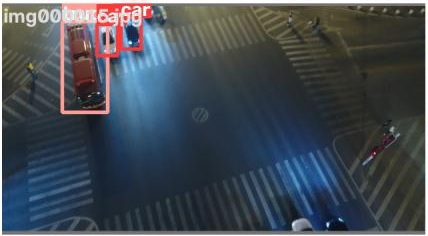
\includegraphics[width=\linewidth]{figures/uavdt-img000015/img000015-label.jpg}
\end{minipage}\hspace{1.2mm}%
\begin{minipage}[c]{0.468\columnwidth}
  \centering
  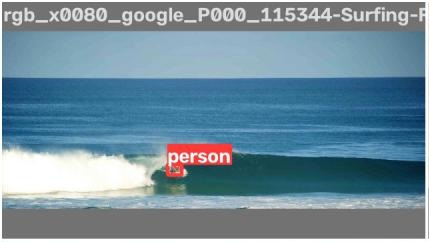
\includegraphics[width=\linewidth]{figures/rgb-x0080-google-115344/rgb-x0080-google-115344-Surfing-label.jpg}
\end{minipage}

\vspace{0.4mm}
% Row 2: ESOD (Baseline)
\begin{minipage}[c]{0.036\columnwidth}
  \centering
  \rotatebox{90}{\scriptsize\textbf{(b) ESOD}}
\end{minipage}\hspace{1mm}%
\begin{minipage}[c]{0.468\columnwidth}
  \centering
  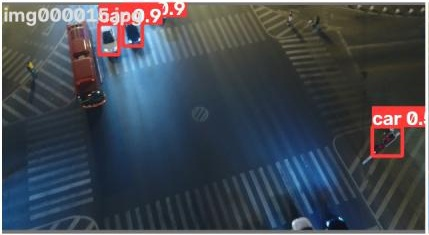
\includegraphics[width=\linewidth]{figures/uavdt-img000015/img000015-esod.jpg}
\end{minipage}\hspace{1.2mm}%
\begin{minipage}[c]{0.468\columnwidth}
  \centering
  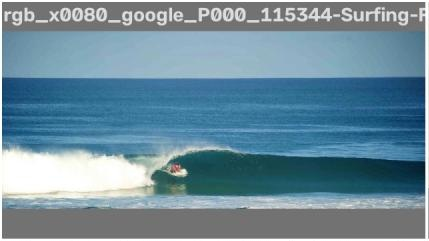
\includegraphics[width=\linewidth]{figures/rgb-x0080-google-115344/rgb-x0080-google-115344-Surfing-esod.jpg}
\end{minipage}

\vspace{0.4mm}
% Row 3: HESOD (Ours)
\begin{minipage}[c]{0.036\columnwidth}
  \centering
  \rotatebox{90}{\scriptsize\textbf{(c) HESOD}}
\end{minipage}\hspace{1mm}%
\begin{minipage}[c]{0.468\columnwidth}
  \centering
  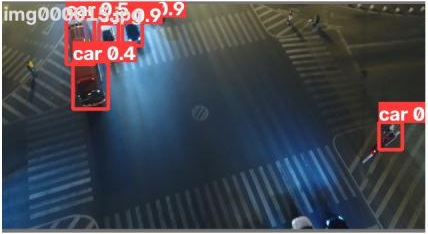
\includegraphics[width=\linewidth]{figures/uavdt-img000015/img000015-hesod.jpg}
\end{minipage}\hspace{1.2mm}%
\begin{minipage}[c]{0.468\columnwidth}
  \centering
  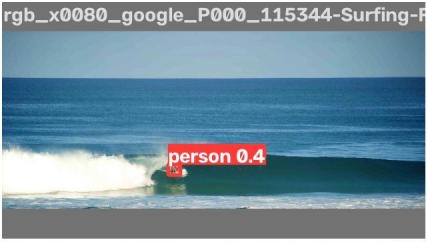
\includegraphics[width=\linewidth]{figures/rgb-x0080-google-115344/rgb-x0080-google-115344-Surfing-hesod.jpg}
\end{minipage}
\vspace{-2.5mm}
\caption{Visual comparison on UAVDT and SeaPerson. Baseline ESOD drops micro targets (b), while HESOD restores full instance recall (c).}
\label{fig:teaser}
\end{figure}

However, spatial selection operates under a severe \emph{asymmetric error cost}: false-positive background patches merely incur minor compute overhead, whereas discarding a true tiny target produces an \emph{irrecoverable false negative}. Existing detectors rely on single semantic objectness with independent per-cell BCE. Under extreme downsampling, micro targets suffer severe semantic collapse, causing faint instances to be prematurely pruned (Fig.~\ref{fig:teaser}(b)). To overcome this recall dilemma, we observe that tiny targets retain high-frequency spatial gradients and spectral saliency even when deep semantics fade~\cite{SET,Guo2025DualDomain,Zhao2025TGRS}. We then propose High-Resolution Efficient Small Object Detection (\textbf{HESOD}) to establish recall-safe, evidence-preserving sparse routing. By coupling dual-evidence routing with an object-level soft-coverage loss, our selector reliably rescues these dropped targets (Fig.~\ref{fig:teaser}(c)). Our contributions include:
\begin{enumerate}\setlength{\itemsep}{0pt}\setlength{\parskip}{0pt}\setlength{\topsep}{1pt}
    \item \textbf{Dual-Evidence Spatial Routing}: We uncover single-semantic routers' vulnerability to feature collapse, coupling semantic objectness with constant-width gradient filtering for scale-robust structural priors independent of backbone capacity.
    \item \textbf{Evidence Preservation and Soft Coverage}: We formulate a monotonic max-fusion rule preventing multi-cue evidence dilution, paired with an object-level noisy-OR soft-coverage loss directly optimizing joint instance recall.
    \item \textbf{Compute Compensation and Empirical Gains}: We co-design an ISPP head that reduces detector parameters by \textgreater27\% while improving $\mathrm{mAP@.5}$ by 0.9/2.3\,pp on UAVDT and SeaPerson, boosting total instance recall by 3.66/3.33\,pp.
\end{enumerate}

\begin{figure*}[t]
\centering
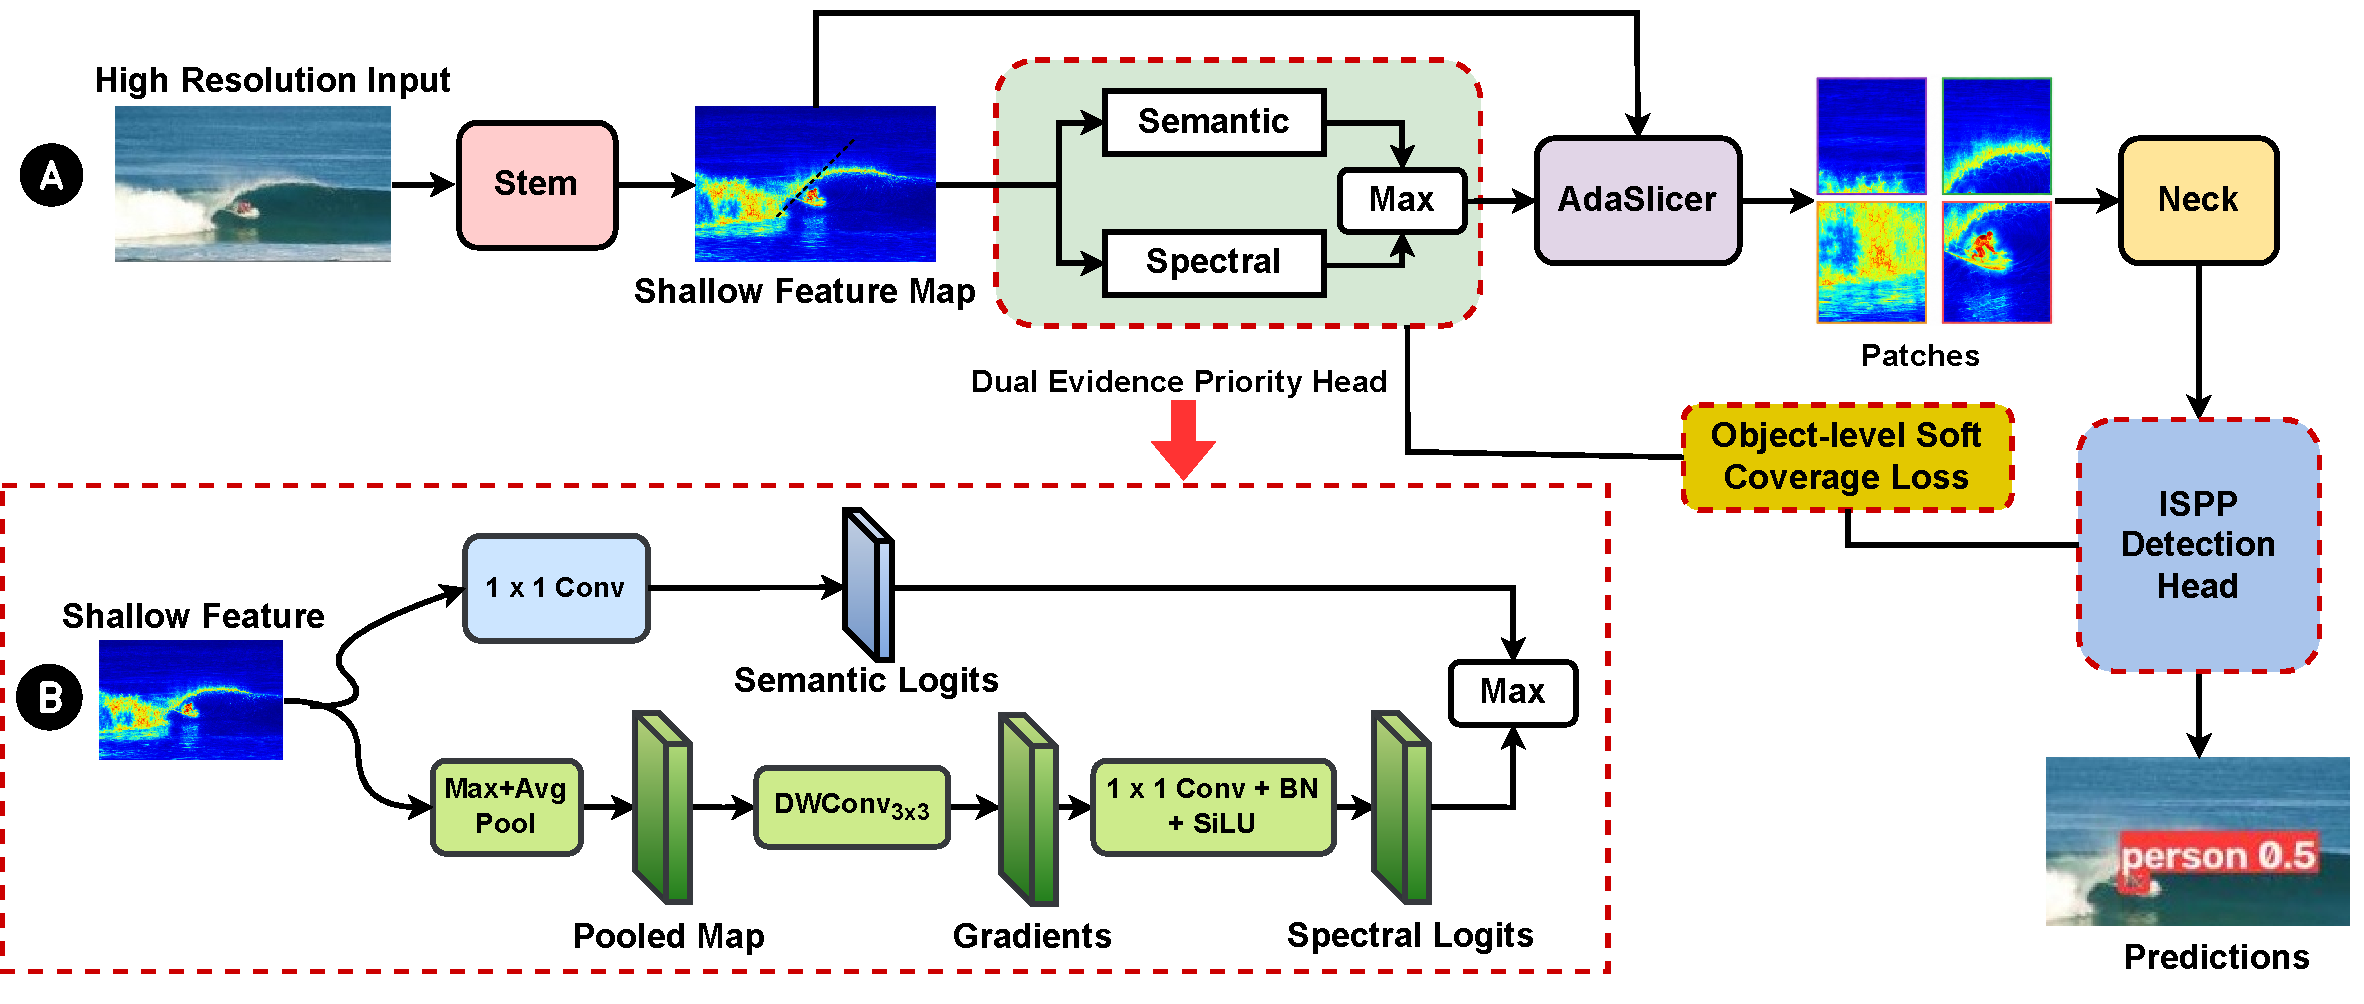
\includegraphics[width=0.90\textwidth]{figures/HESOD.pdf}
\vspace{-2.5mm}
\caption{Overview of HESOD: (a) End-to-end selective pipeline; (b) Dual-Evidence Priority Head. Red dashed boxes highlight our proposed contributions over ESOD.}
\label{fig:overview}
\end{figure*}
